\chapter{Installing and Running Gmsh}
\thispagestyle{empty}
\label{sec:chap4}
\newcommand{\LocCHfourfig}{\Origin/CHAPTERS/chap4/figures}

Gmsh is a Free and Open Source three dimensional finite element grid generator with a build-in CAD engine and post-
processor. There are four modules available in Gmsh such as Geometry, Meshing, Solver and Post-Processiing. Using
Gmsh we can mesh the geometry and import it in OpenFOAM using the mesh conversion utilities (see chapter 17 for more info).
In this chapter we will cover how to install Gmsh and create a simple geometry.It is expected that the user should have knowledge 
about Meshing.

\section{Installing Gmsh}

Gmsh can be installed using Synaptic Package Manager. Open Gmsh in your system by typing your system passowrd.
In the search box type Gmsh and install it, Fig \ref{synaptic-gmsh}. This might take some time depending on your internet speed.

\begin{figure}[ht]  
\begin{center}  
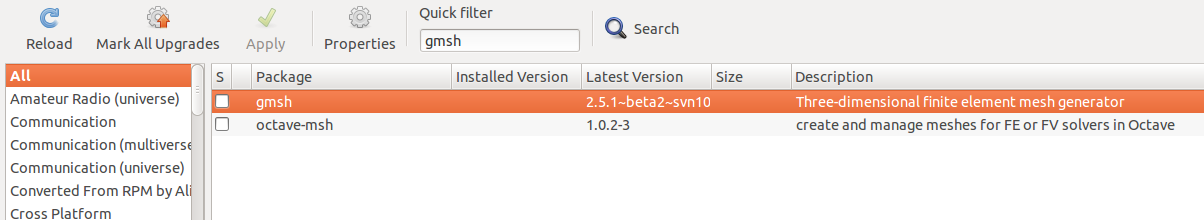
\includegraphics[scale=0.32]{\LocCHfourfig/synaptic-gmsh.png}
\caption{Install Gmsh}
\label{synaptic-gmsh}
\end{center}  
\end{figure}


\flushleft Alternately we can also install Gmsh from the gmsh website given below,

\center {\textbf{http://geuz.org/gmsh/}} \newline

\flushleft Open this website in your browser and scroll down to download. Now Download Gmsh according to the given current stable release 
Fig \ref{download-gmsh} according to your Operating System (OS).

\begin{figure}[ht]  
\begin{center}  
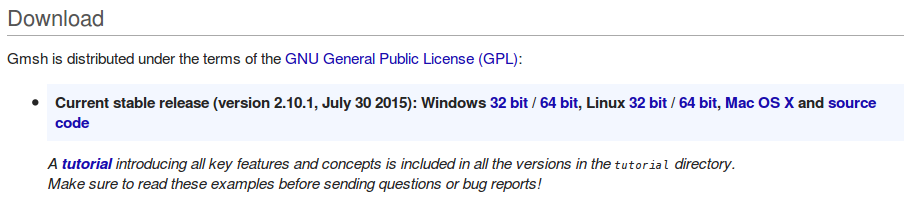
\includegraphics[scale=0.352]{\LocCHfourfig/download-gmsh.png}
\caption{Download stable release}
\label{download-gmsh}
\end{center}  
\end{figure}

\begin{figure}[ht]  
\begin{center}  
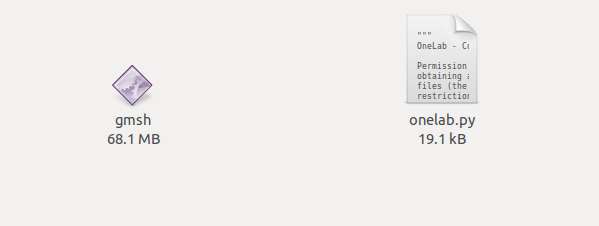
\includegraphics[scale=0.26]{\LocCHfourfig/gmsh-icon.png}
\caption{gmsh-icon}
\label{gmsh-icon}
\end{center}  
\end{figure}


\flushleft In the Download folder extract the downloaded gmsh tar file. After you open the folder you will see folder named bin, click on it. 
Inide the bin folder you will see the Gmsh icon, Fig \ref{gmsh-icon}. Double click on it to launch the Gmsh Start screen, Fig \ref{gmsh-start} \newline

As a pracice to learn Gmsh we will create a cube of sides 1 unit as seen in the Fig, \ref{geometry1}. On the left hand side in the Gmsh window you can 
see three modules namely,

\begin{itemize}
\item Geometry
\item Mesh
\item Solver
\end{itemize}

Click on the Geometry module, then go to Elementary Entities, inside elementary entities go to add and then click on points. This will open up a
window where you can enter the X, Y and Z co-ordinates starting with 0 inside each box and press Enter, Fig \ref{point}. Now
enter points for all the remaining 7 vertices to complete the cube, Fig \ref{geometry1}. In the Gmsh screen we can see the eight points, you can move those points
using the left mouse click. To join these points click on Straight-line option under Elementary Entities. Now select any two points to create a straight line, click 
on the start point and then the second point to create a line. Similarly join all the other points to create a cube as shown in the Fig, \ref{line} below.
As you can see on the Gmsh screen you can press e to end selection and q to abort.

\begin{figure}[t]  
\begin{center}  
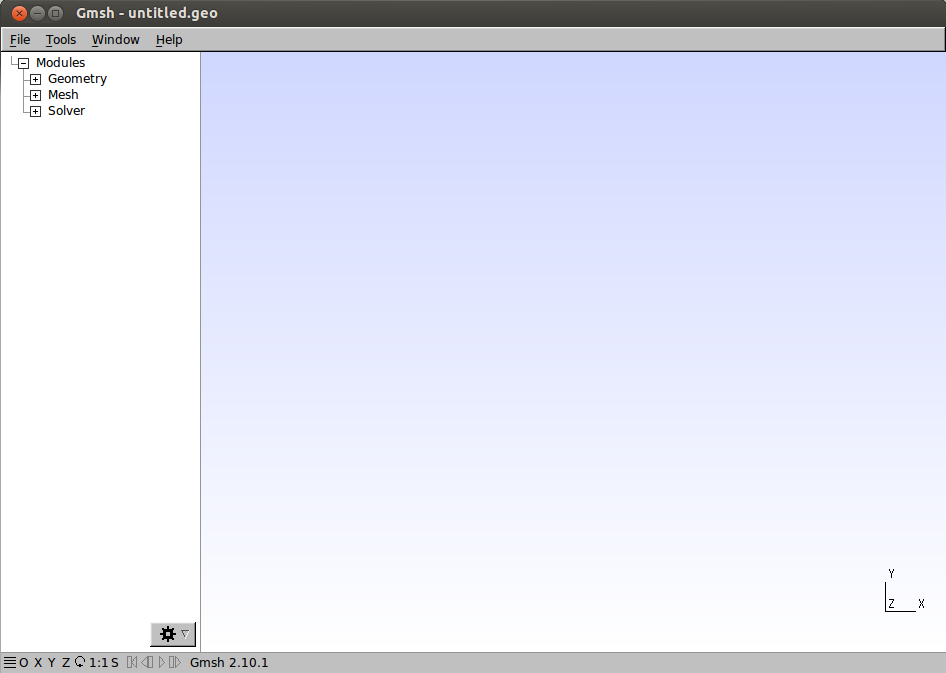
\includegraphics[scale=0.28]{\LocCHfourfig/gmsh-start.png}
\caption{gmsh-icon}
\label{gmsh-start}
\end{center}  
\end{figure}

\begin{figure}[t]  
\begin{center}  
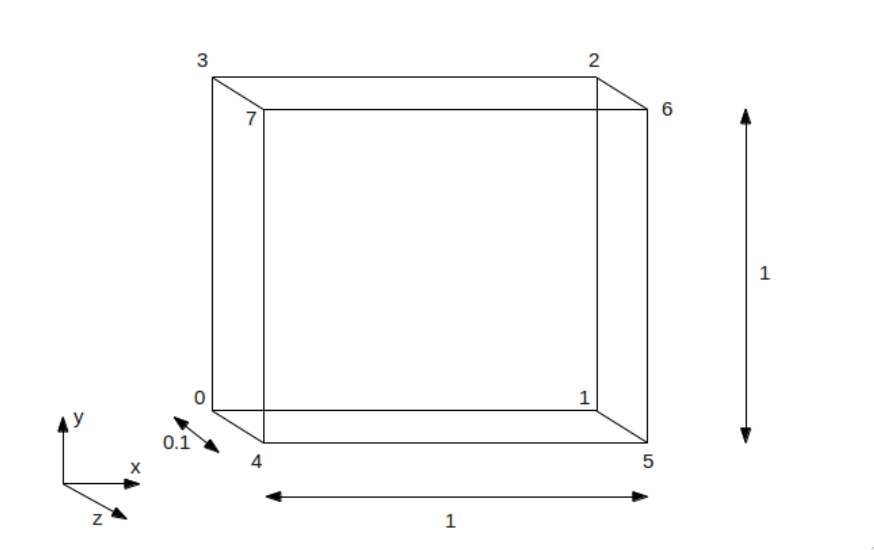
\includegraphics[scale=0.28]{\LocCHfourfig/geometry1.png}
\caption{Cube of unit dimension}
\label{geometry1}
\end{center}  
\end{figure}

\begin{figure}[t]  
\begin{center}  
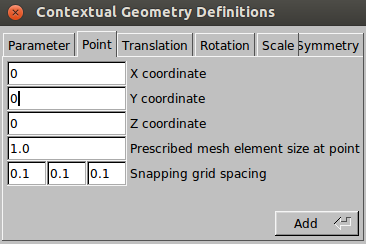
\includegraphics[scale=0.28]{\LocCHfourfig/point-gmsh.png}
\caption{Points window}
\label{point}
\end{center}  
\end{figure}

\begin{figure}[t]  
\begin{center}  
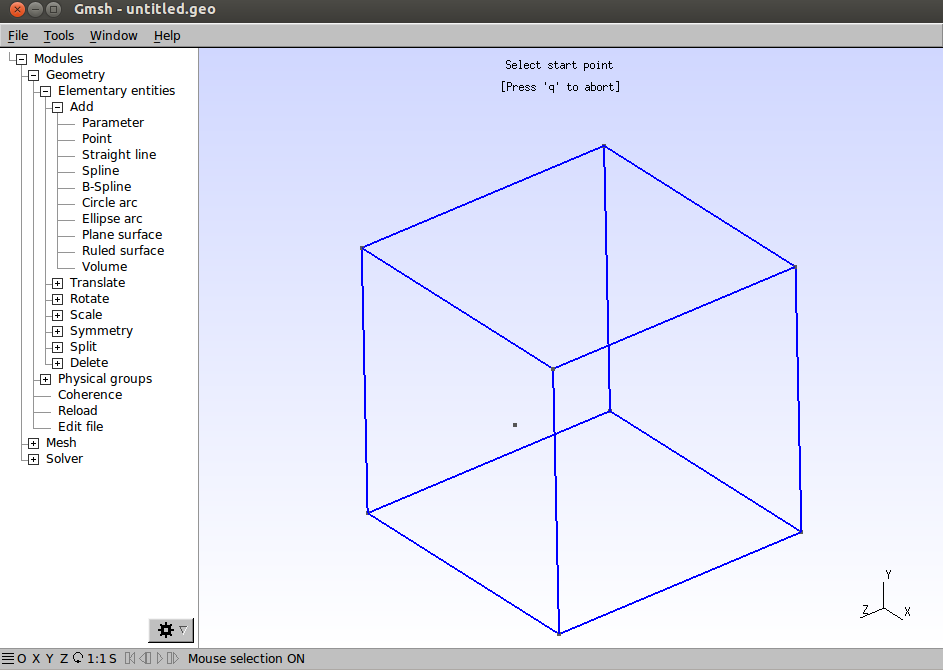
\includegraphics[scale=0.28]{\LocCHfourfig/cube-gmsh.png}
\caption{Join the points using line}
\label{line}
\end{center}  
\end{figure}

\subsection{Create Faces}

To create faces for the cube click on plane-surface unde elementery enetities. After this select the outer booundaries of the face of a rectangle.
Select the edges of the bottom face first.Once you select the edges they will turn red in color, Fig \ref{face}. Check in case if there is any hole in the 
face, if none then press e to end selection. You will notice that a face will appear with dasshed center lines, Fig \ref{cl}. Repeat this procedure for 
remaining faces, Fig \ref{face-all} and finally press q to abort.

\begin{figure}[t]  
\begin{center}  
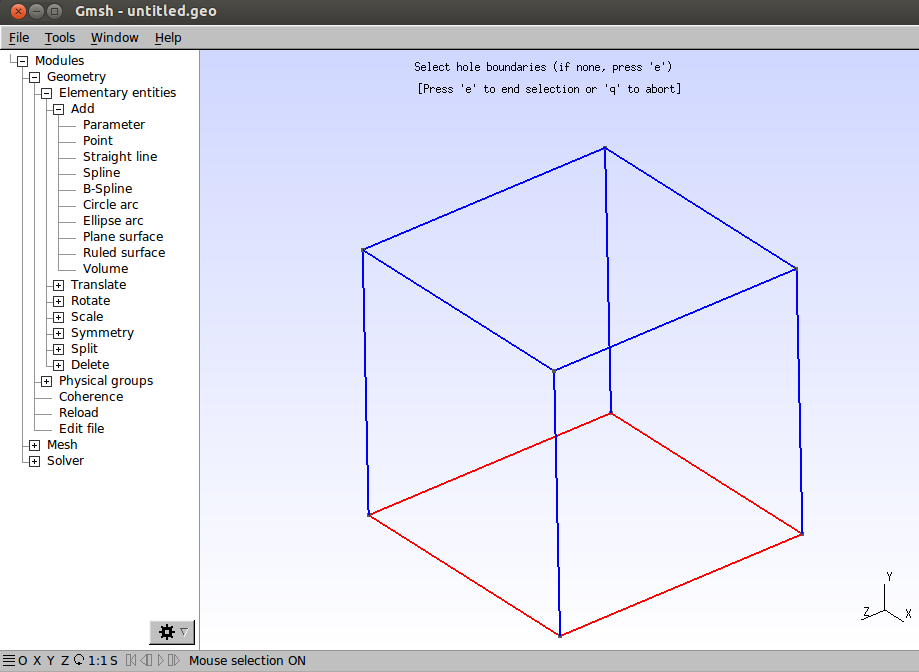
\includegraphics[scale=0.28]{\LocCHfourfig/face-red.png}
\caption{Selct edges}
\label{face}
\end{center}  
\end{figure}


\begin{figure}[t]  
\begin{center}  
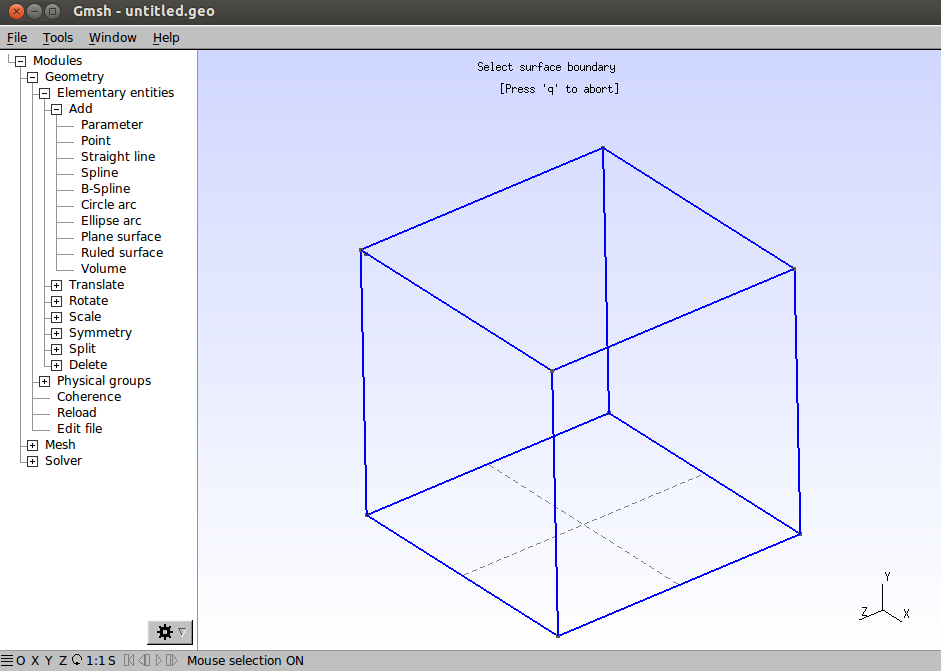
\includegraphics[scale=0.28]{\LocCHfourfig/face-cl.png}
\caption{Bottom Face}
\label{cl}
\end{center}  
\end{figure}

\begin{figure}[t]  
\begin{center}  
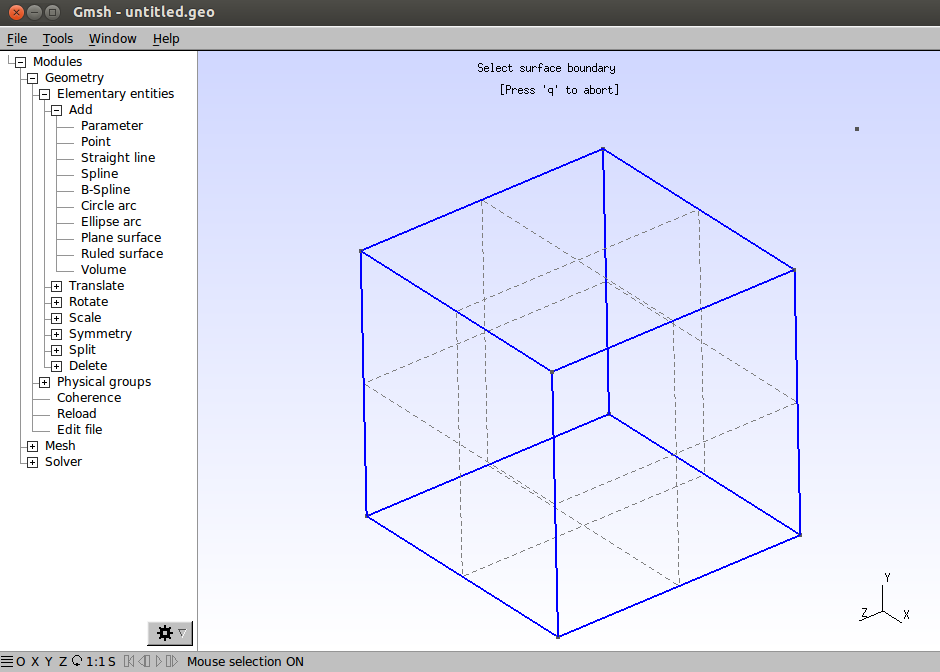
\includegraphics[scale=0.28]{\LocCHfourfig/face-all.png}
\caption{Create faces for all surfaces}
\label{face-all}
\end{center}  
\end{figure}

\subsection{Creating Volume}

We now need to create volume boundary. We need to select the Volume boundary similar to selecting boundary for faces. 
Click on the Volume boundary under elementery entities and click on boundary surface of the cube and press e to end selection. A yellow dot will
appear at the center of the cube which represents volume in Gmsh. Press q to abort the selction.

\begin{figure}[t]  
\begin{center}  
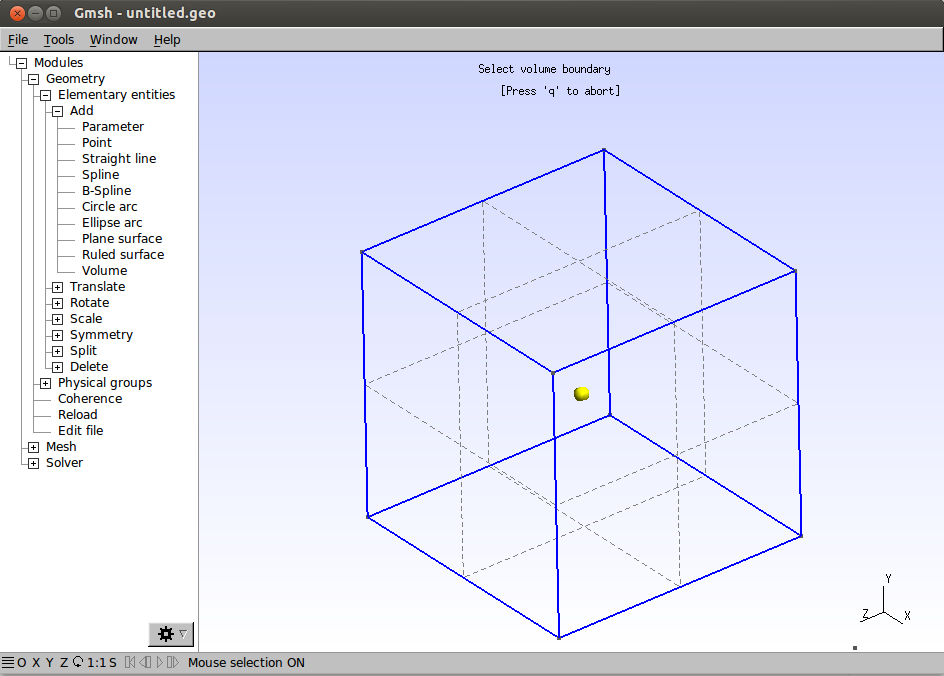
\includegraphics[scale=0.28]{\LocCHfourfig/vol-gmsh.png}
\caption{Volume}
\label{vol}
\end{center}  
\end{figure}

\subsection{Physical Groups}

In Gmsh we need to create physical groups which will be useful for exporting the Mesh file to OpenFOAM. To do so click on Physical Group under Geometry Module.
Click on Add and then Surface. Upon selection of any face it will turn red. Now press e to end selection. Do this procedure for all the remaining faces
and press q to abort. Also we need to select the Physical Volume. Click on Volume under Physical Groups and select the yellow dot at the center of the cube.
The yellow dot will turn red in colora dn press e to end selection and q to abort.

To save the geometry under the file menu click on Save as and save the geometry by the name cube.geo. Here "geo" stands for geometry. Click OK twice
to save the geometry. 


